\section{互熵与互信息}
前面我们给出了熵、联合熵、条件熵的定义与性质, 这些熵都是概率分布不肯定性的度量. 这一节我们给出两个概率分布 “差异性” 的度量值, 且把这种 “差异性” 的度量也看成一种信息量.

\subsection{互熵}
\begin{definition}
    设 $ p(x), q(x) $ 是 $ \mathscr{X} $ 上的两个概率分布, 它们的互熵定义为
$$
H(p \| q)=\sum_{x \in \mathscr{X}} p(x) \log \frac{p(x)}{q(x)}
$$
规定 $ 0 \log \frac{0}{0}=0 $, 另外, 如有一个 $ x \in \mathscr{X} $ ,使 $ p(x)=0 $ ,而 $ q(x)>0 $, 那么规定 $ H(p \| q)=\infty $.
\end{definition}
 \begin{remark}
     (1)互熵是两个概率分布 “差异性” 的度量;\\
(2) 由上一节引理\ref{lamma2}知 $ H(p \| q) \geqslant 0 $;\\
(3) $ H(p \| q)=0 \Leftrightarrow$ 对于$p(x) \neq 0 $的$x$均有 $p(x)=q(x)$.
 \end{remark}
\begin{example}
设 $ \mathscr{X}=\left\{x_{1}, x_{2}, x_{3}\right\} $, 以等概率 $ p_{i}=\frac{1}{3} $ 和以概率 $ q_{1}=q_{2} $ $ =\frac{1}{4}, q_{3}=\frac{1}{2} $ 从 $ \left\{x_{1}, x_{2}, x_{3}\right\} $ 中抽样, 这两个概率分布的互熵是多少?
$$
\begin{aligned}
H(p \| q) & =\sum_{x \in \mathscr{X}} p(x) \log \frac{p(x)}{q(x)}=\sum_{i=1}^{3} p_{i} \log \frac{p_{i}}{q_{i}} \\
& =\frac{1}{3} \log \frac{1 / 3}{1 / 4}+\frac{1}{3} \log \frac{1 / 3}{1 / 4}+\frac{1}{3} \log \frac{1 / 3}{1 / 2} \\
& =\frac{1}{3} \log \frac{4}{3} \times \frac{4}{3} \times \frac{2}{3}=\frac{1}{3} \log \frac{32}{27} \\
& =\frac{5}{3}-\frac{1}{3} \log 27=\frac{5}{3}-\frac{1}{3} \log 3^{3} \\
& =\frac{5}{3}-\log 3 \approx \frac{5}{3}-1.585=0.082
\end{aligned}
$$
\end{example}

\subsection{互信息}
\begin{definition}
    对于两个随机变量 $ \xi $ 与 $ \eta $, 它的联合分布为 $ p(x, y) $, 边际分布为 $ p(x) $ 与 $ q(y) $ ,则 $ \xi $ 与 $ \eta $ 的互信息 $ I(\xi ; \eta) $ 定义为:
$$
\begin{aligned}
I(\xi ; \eta) & =H(p(x, y) \| p(x) q(y)) \\
& =\sum_{x \in \mathscr{X}} \sum_{y \in \mathscr{Y}} p(x, y) \log \frac{p(x, y)}{p(x) q(y)}
\end{aligned}
$$
\end{definition}

\begin{theorem}
    由互信息 $ I(\xi ; \eta) $ 的定义可知如下性质成立:\\
(1) 对称性: $ I(\xi ; \eta)=I(\eta ; \xi) $;\\
(2) 互信息与联合熵及条件熵的关系为
$$
\begin{array}{l}
I(\xi ; \eta)=H(\xi)+H(\eta)-H(\xi, \eta) ; \\
I(\xi ; \eta)=H(\xi)-H(\xi \mid \eta) ; \\
I(\xi ; \eta)=H(\eta)-H(\eta \mid \xi) ;
\end{array}
$$
(3)非负性:对任何随机变量 $ \xi, \eta $, 总有 $ I(\xi ; \eta) \geqslant 0 $, 等号成立的充要条件为 $ \xi $ 与 $ \eta $ 是相互独立的随机变量;\\
(4)如果 $ f $ 是从 $ \mathscr{Y} $ 到 $ \mathscr{Z} $ 的任意映射,那么必有 $ I(\xi ; \eta) \geqslant I(\xi ; f(\eta)) $, 等号成立的充要条件为 $ f $ 是一个 $ 1-1 $ 变换;\\
(5) $ I(\xi, \xi)=H(\xi) . $

\end{theorem}
\begin{proof}
(1)显然;

(2)
$$
 \begin{aligned}
& I(\xi ; \eta)=\sum_{x \in \mathscr{X}} \sum_{y \in \mathscr{Y}} p(x, y) \log \frac{p(x, y)}{p(x) q(y)} \\
= & \sum_{x \in \mathscr{X}} \sum_{y \in \mathscr{Y}} p(x, y)[\log p(x, y)-\log p(x) q(y)] \\
= & \sum_{x \in \mathscr{X}} \sum_{y \in \mathscr{Y}} p(x, y)[\log p(x, y)-\log p(x)-\log q(y)] \\
= & \sum_{x \in \mathscr{X}} \sum_{y \in \mathscr{Y}} p(x, y) \log p(x, y)-\sum_{x \in \mathscr{X}} \sum_{y \in \mathscr{Y}} p(x, y) \log p(x)  -\sum_{x \in \mathscr{X}} \sum_{y \in \mathscr{Y}} p(x, y) \log q(y) \\
= & -H(\xi, \eta)+H(\xi)+H(\eta)=H(\xi)+H(\eta)-H(\xi, \eta)
\end{aligned}
$$
而
$$
\begin{array}{l}
H(\xi, \eta)=H(\eta)+H(\xi \mid \eta) \\
H(\xi, \eta)=H(\xi)+H(\eta \mid \xi)
\end{array}
$$
于是有
$$
I(\xi ; \eta)  =H(\xi)+H(\eta)-[H(\eta)+H(\xi \mid \eta)]  =H(\xi)-H(\xi \mid \eta)
$$
和 $$ I(\xi ; \eta)=H(\xi)+H(\eta)-[H(\xi)+H(\eta \mid \xi)]
=H(\eta)-H(\eta \mid \xi)
$$

(3)显然;
(4)类似于定理\ref{the3}可证;

(5)
$$
\begin{aligned}
I(\xi, \xi) & =\sum_{x \in \mathscr{X}} p(x) \log \frac{p(x)}{p(x) p(x)} \\
\quad= & -\sum_{x \in \mathscr{X}} p(x) \log p(x)=H(\xi)
\end{aligned}
$$
\end{proof}

\subsection{条件互信息}
\begin{definition}
    随机变量 $ \xi $ 与 $ \eta $ 在给定随机变量 $ \zeta $ 时的条件互信息定义为
$$
\begin{aligned}
I(\xi ; \eta \mid \zeta) & =H(p(x, y \mid z) \| p(x \mid z) \cdot p(y \mid z)) \\
& =\sum_{(x, y, z) \in \mathscr{X} \otimes \mathscr{Y} \otimes \mathscr{Z}} p(x, y \mid z) \log \frac{p(x, y \mid z)}{p(x \mid z) p(y \mid z)}
\end{aligned}
$$
\end{definition}

条件互信息与条件熵的关系为
$$
\begin{aligned}
I(\xi ; \eta \mid \zeta) & =H(\xi \mid \zeta)+H(\eta \mid \zeta)-H(\xi, \eta \mid \zeta) \\
& =H(\xi \mid \zeta)-H(\xi \mid \eta, \zeta) \\
& =H(\eta \mid \zeta)-H(\eta \mid \xi, \zeta)
\end{aligned}
$$
\begin{example}
    设有一信源输出 $ \mathscr{X}=\{0,1,2\} $, 其概率为 $ p_{0}=\frac{1}{4} $, $ p_{1}=\frac{1}{4}, p_{2}=\frac{1}{2} $, 设计一个实验去观察, 其结果为 $ \mathscr{Y} \in\{0,1\} $,已知条件概率为
    \begin{table}[h]
        \centering
\begin{tabular}{c|c|c}
\hline$ p(y \mid x) $ & 0 & 1 \\
\hline 0 & 1 & 0 \\
\hline 1 & 0 & 1 \\
\hline 2 & $ \frac{1}{2} $ & $ \frac{1}{2} $ \\
\hline
\end{tabular}
\end{table}
求 $ I(\mathscr{X} ; \mathscr{Y}) $ .

解:对于 $ \mathscr{Y} $
$$
\begin{aligned}
p(y & =0)=\sum_{i=0}^{2} p\left(x_{i}, y=0\right) \\
& =\sum_{i=0}^{2} p\left(x_{i}\right) p\left(y=0 \mid x_{i}\right) \\
& =p(0) p(y=0 \mid 0)+p(1) p(y=0 \mid 1)+p(2) p(y=0 \mid 2) \\
& =\frac{1}{4} \times 1+\frac{1}{4} \times 0+\frac{1}{2} \times \frac{1}{2} \\
& =\frac{1}{2}
\end{aligned}
$$
$$ \begin{aligned} p(y & =1)=\sum_{i=0}^{2} p\left(x_{i}, y=1\right) \\ & =\sum_{i=0}^{2} p\left(x_{i}\right) p\left(y=1 \mid x_{i}\right) \\ & =p(0) p(y=1 \mid 0)+p(1) p(y=1 \mid 1)+p(2) p(y=1 \mid 2) \\ & =\frac{1}{4} \times 0+\frac{1}{4} \times 1+\frac{1}{2} \times \frac{1}{2} \\ & =\frac{1}{2} \\ I(\mathscr{X} & ; \mathscr{Y})=\sum_{x \in \mathscr{X}} \sum_{y \in \mathscr{Y}} p(x, y) \log \frac{p(x, y)}{p(x) p(y)} \\ & =\sum_{x \in \mathscr{X}} \sum_{y \in \mathscr{Y}} p(x) p(y \mid x) \log \frac{p(y \mid x)}{p(y)} \\ & =\frac{1}{4} \times 1 \times \log 2+\frac{1}{4} \log 2+\frac{1}{2} \log 1+\frac{1}{2} \log 1 \\ & =\frac{1}{4}+\frac{1}{4} \\ & =0.5 \text { (比特/符号) }\end{aligned} $$

或者利用$I(\mathscr{X}  ; \mathscr{Y})=H( \mathscr{Y})-H( \mathscr{Y}| \mathscr{X})$,我们计算知$H( \mathscr{Y})=H(\frac 12)=1$,$H( \mathscr{Y}| \mathscr{X})=\frac 14\times 0+\frac 14\times 0+\frac12\times(\frac 12\log 2+\frac 12\log 2)=\frac 12$,于是$I(\mathscr{X}  ; \mathscr{Y})=1-\frac 12=\frac 12$
\end{example}
\subsection{各种熵与互信息之间的关系}
$$
\begin{array}{l}
I(\xi, \eta)=H(\xi)+H(\eta)-H(\xi, \eta) \\
H(\xi \mid \eta)=H(\xi)-I(\xi, \eta) \\
H(\xi, \eta)=H(\xi)+H(\eta \mid \xi) \\
I(\xi, \eta)=H(\eta)-H(\eta \mid \xi)
\end{array}
$$
\begin{figure}[h]
    \centering
    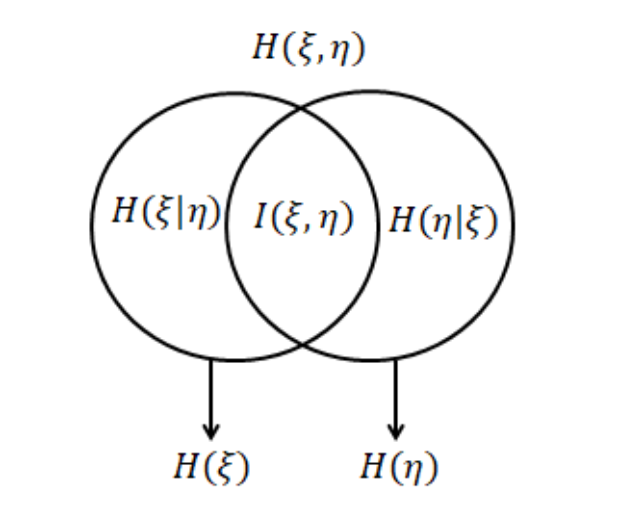
\includegraphics[width=0.4\linewidth]{image/1.png}
\end{figure}




